\documentclass[11pt, a4paper,notitlepage]{article}
\usepackage{amsfonts, amsmath, hanging, hyperref, parskip, times}
%\usepackage[pdftex]{graphicx}
\usepackage{graphicx}
\usepackage[numbers]{natbib}
\setcitestyle{notesep={  }}
\usepackage{inputenc}
%Packages by Giuseppe
\usepackage{float}
%\usepackage{verbatim} This package is replaced by fancyvrb
\usepackage{enumerate}
\usepackage{enumitem}   % for having itemized list with letters
\usepackage{multirow}
\usepackage{listings}
\usepackage{array}
% get package xr for cross referencing
%\usepackage{xr}
%\externaldocument{formality_8pic}
%\externaldocument{readability_8pic}

\usepackage[toc,page]{appendix}   % for creating appendices
\usepackage{tikz}
\usetikzlibrary{arrows,chains,matrix,positioning,scopes}
\usetikzlibrary{arrows,chains,matrix,positioning,scopes}
\usepackage{pgfplots}
%\usepackage{filecontents} 
\usepackage{fancyvrb}  %this package allows to set fontsize in verbatin environment
\usepackage{multirow}
\usepackage[skip=2pt]{caption}
\usepackage[skip=0pt]{subcaption}
\captionsetup[figures]{skip=0pt}
%\usepackage{tabularx}
\DeclareCaptionFont{tiny}{\tiny}
\usepackage{tikz}
\usetikzlibrary{calc,trees,positioning,arrows,chains,shapes.geometric,%
    decorations.pathreplacing,decorations.pathmorphing,shapes,%
    matrix,shapes.symbols}
% define the expectation operator
\DeclareMathOperator{\E}{\mathbb{E}}  

%\hypersetup{
%  colorlinks,
%  linkcolor=blue,
%  urlcolor=blue
%}

% \let\section=\subsubsection
\newcommand{\pkg}[1]{{\normalfont\fontseries{b}\selectfont #1}} 
\let\proglang=\textit
\let\code=\texttt 
\renewcommand{\title}[1]{\begin{center}{\bf \LARGE #1}\end{center}}
\newcommand{\affiliations}{\footnotesize}
\newcommand{\keywords}{\paragraph{Keywords:}}

\setlength{\topmargin}{-15mm}
\setlength{\oddsidemargin}{-2mm}
\setlength{\textwidth}{165mm}
\setlength{\textheight}{250mm}

\begin{document}

\pagestyle{empty}

\title{Text Mining and Sentiment Extraction in Central Bank Documents}
{
\begin{center}

\vspace*{\stretch{0.8}} \par
\vspace*{\stretch{1.6}}

\Large
{\bf Giuseppe Bruno$^*$} \\[2mm]
\normalsize
Bank of Italy, Economics and Statistics Directorate.
\par
\vspace*{\stretch{1.5}}
\begin{abstract}
The deep transformation induced by the World Wide Web (WWW) revolution has thoroughly impacted  a relevant part
of the social interactions in our present {\it global society}. The huge amount of unstructured information available on
blogs, forum and public institution web sites puts forward different challenges and opportunities.
%The ease with which opinion survey can be conducted and the possibility to scrape for unsolicited comments on 
%particular  subjects offer new avenues for statistical evaluation of level of satisfaction for a given service
%and the size of consensus with respect to a social choice.
Starting from these considerations, in this paper we pursue a two-fold goal.
Firstly we review some of the main methodologies employed in
text mining and for the extraction of sentiment and emotions from textual sources. 
Secondly we provide an empirical application by considering the latest 20 issues of the Bank of Italy
{\it Governor's concluding remarks} from 1996 to 2015. 
By taking advantage of the open source software package {\proglang R}, 
we show the following:
\begin {enumerate}
\item checking the word frequency distribution features of the documents;
\item extracting the evolution of the sentiment and the polarity orientation in the texts;
\item evaluating the evolution of an index for the readability and the formality level of the texts;
\item attempting to measure the popularity gained from the documents in the web. 
\end{enumerate}
The results of the empirical analysis show the feasibility in extracting the main 
topics from the considered corpus. Moreover it is shown how to check
for positive and negative terms in order to gauge the polarity of statements and whole documents.
Although \proglang{R}, the employed software, has proved suitable and comprehensive 
 for the required tasks, the whole
picture presents lights and shadows. Improvements in the documentation and 
the package arrangement and portability  among platforms are suggested in the text.
   
 
% I should arrive on line 78 for the abstract.
%\vspace{0.3cm} \newline
\vskip 0.5cm
\vspace{0.3cm}

\noindent{ \emph{JEL classification}: C83, E58, E66.}
\newline
\noindent{ \emph{Keywords}: Text Mining, Wordcloud, Polarity, Sentiment Analysis, Zipf's Law.}
\vskip 0.5cm
\vspace{0.3cm}

\end{abstract}
\vspace*{\stretch{1.5}}

\end{center}
\vspace*{\stretch{0.5}}

%\footnotesize \renewcommand{\baselinestretch}{0.6}
%\rule{2in}{1pt}
%\\ \renewcommand{\baselinestretch}{0.2}
%\begin{center}
\begin{affiliations}
1. Bank of Italy, Research Area. \\[-2pt]
$^\star$ \href{mailto:giuseppe.bruno@bancaditalia.it}{giuseppe.bruno@bancaditalia.it}\\[-2pt]
This version December 2015 \\[-2pt]
The author wishes to thank Roberto Stok for his helpful suggestions and unceasing cooperation.\\[-2pt]
The views expressed are the author's only and do not imply those of  the Bank of Italy.\\[-2pt]

\end{affiliations}

\newpage
\thispagestyle{empty}
\pagestyle{plain}
\setcounter{page}{2}
\pagenumbering{arabic}

\mbox{}
\

\section{Introduction and motivation}
\null\vspace{\stretch{1}}
\begin{flushright}
{\footnotesize {\it A big computer, a complex algorithm and a long\\
 time does not equal science.}} {\scriptsize -- Robert Gentleman}
\end{flushright}
\vspace{\stretch{2}}\null
The deep transformation caused by the World Wide Web (WWW) revolution has 
thoroughly impacted  a relevant part of social interactions. 
According to \href{http://www.internetlivestats.com}{{\it www.internetlivestats.com}} on August 20 of 2015, we had
 more the 3.1 billion of Internet users visiting almost 1 billion websites. Moreover
there were about 1.5 billion of Facebook active users and approximately 900 million Tweets per day. 
The final upshot of these numbers is that we end up with a
huge amount of unstructured textual information available on
blogs, forum and public institution web sites which  puts forward different challenges and opportunities.
According to recent estimates about 4/5 of the whole set of web pages is composed of textual information.
Mining valuable information out of a corpus of many documents, classifying sentiment or even providing a
polarity measure on a given topic is an already widely applied technique in different fields such as
marketing, social and political networks. 
Although their popularity in these fields, text mining and sentiment analysis have just recently shown 
up on the tool repertoire of Central bank's economists (for an overview of the problem 
see \citet{Bholat2015}).
Text mining consists in building a sound synthesis from a set of documents, often referred as a corpus,  
that allow to quickly carry out the following tasks:
\begin{enumerate}[label=\alph* )]
\item  allocate the text to a given semantic category;
\item  evaluate the word frequency distribution in the text;
\item  verify global statistical features of the considered text;
\end{enumerate} 

%To mine text, we first need to process it into a form that text-mining procedures can use. 
The sentiment analysis 
is a follow up task aimed at designing automatic procedures for opinion discovery and summarization system
from a set of textual information (\citet{Bing2010} presents a thorough and formal analysis on the topic).  
There we  find a clear definition of the sentiment analysis as the computational study of opinions and emotions 
expressed in textual document. Moreover it is introduced a dichotomy  between direct and comparative opinions which
are the goal of the investigation. Text minining has also been considered by \citet{Hendry2010} 
for the Bank of Canada communications. 
Here the authors put forth the {\it Latent Semantic Analysis} (LSA)
to extract relevant meanings from Bank of Canada communications \footnote {LSA is a technology 
widely used in internet search engines. It is based on the application of a Singular Value Decomposition on the 
term-document matrix obtained from the considered corpus.}.    

 Our work provides some useful insights on the actual capability to start dealing with textual information in order to
 gauge sentiment orientation and possibly some polarity evaluation for broadening the set of our 
statistical collection tools. In particular, with reference to our corpus composed of a set of the Bank of 
Italy Governor's {\it Concluding Remarks},  this work attempts 
to answer the following questions:

\begin{enumerate}
\item[1)]  what are the features of the word frequency distributions of the texts?
\item[2)]  what is the sentiment orientation and the polarity value?
\item[3)]  what is the readability and formality level?
\item[4)]  what is the interest/memorability  gained from the documents in our corpus?
\end{enumerate} 
 
   
The recent literature on these themes (see for example \citet{Bholat2015} and \citet{Nyman2015}) witnesses the growing interest
shown by other Central Banks on these issues and that one closely linked with the emergence of the
 {\it Big Data} theme. 

The appearance of web tools for monitoring social media by semantic and sentiment orientation, 
provides analytical support fostering a wider adoption of text mining techniques for implementing
well informed decisions. 
 
This paper is arranged in the following way. After this introduction 
in  section~\ref{sec:Corpus_Text}  we present the basic theoretical concepts behind the text-mining techniques. 
Section ~\ref{sec:Graphic_Tool} presents some graphical tools widely employed to show the main concepts contained in the 
examined document. Section~\ref{sec:Stat_Laws} introduces the two relevant computational 
linguistic statistics allowing to compare and check the stability of these synthetic measure over time.
Section~\ref{sec:Empirical_application} presents some results of this statistical analysis carried out 
on a corpus containing the last 20 editions, from 1996 to 2015, of the {\it Governor's Concluding Remarks}.
Finally section ~\ref{sec:Conclusion} provides some concluding remarks.
  
\vskip 0.8cm


\section {Analysing a corpus of Text documents}
\label{sec:Corpus_Text}

Textual data provides a huge and diversified range of information. Nonetheless 
this information is encoded in a way that doesn't lend itself to an automatic 
deciphering step.
Since about three decades,  computational linguistics
has tried to take advantage of  large text collections
in order to design text analysis algorithms. Text mining is a broad umbrella term illustrating a
wide range of technologies for analyzing textual data which are intrinsically unstructured.

Following the suggestions in \citet{Hearst1999}
we define text mining as the task of  harnessing {\it a large online
text collections to discover new facts and trends about the world itself}. 

The task of analysing  a corpus of text can be grasped by looking at the
 diagram in figure \ref{tm_scheme1}:
%% Author: Giuseppe Bruno
\begin{figure}[ht]
\begin{tikzpicture}[node distance=4mm, >=latex',
 block/.style = {draw, rectangle, minimum height=10mm, minimum width=28mm,align=center,rounded corners=.5em},
 bigblock/.style = {draw, rectangle, minimum height=14mm, minimum width=34mm,align=center,rounded corners=0.5em},
rblock/.style = {draw, rectangle, rounded corners=0.5em},
                        ]
    \node [bigblock]                    (start)     {Text collection \\ Corpus};
    \node [block, below=of start]       (encode)    {Get text encoding\\ Latin1,UTF-8};
    \node [block, right=of encode]     (lang_det)   {Language detection};
    \node [block, right=of lang_det]    (xtract)      {Layout and component\\ removal};
    \node [block, below=of lang_det]    (Tokeniz)  {Tokenization\\ text segmentation};
    \node [block, below=of Tokeniz]    (Stword)   {Stop word removal};
    \node [block, below=of Stword]     (stemm) {Conflation: stemming\\ lemmatization};
    \node [block, below=of stemm]      (postag)     {Part of Speech POS\\ tagging};
    \node [block, below=of postag]     (homo)     {homonymous \& \\ synonymous recognition};
    \node [block, below left=of homo]  (semant)     {Semantics \\ Sentiment analysis};
    \node [block, below right=of homo] (word)     {Wordcloud \& \\ word histogram};


%% paths 
    \path[draw,->] (start)    edge  (encode)
                   (encode)   edge  (lang_det)
                   (lang_det) edge  (xtract)
                   (xtract)   |-  (Tokeniz)
                   (Tokeniz)  edge  (Stword)
                   (Stword)   edge  (stemm)
                   (stemm)    edge  (postag)
                   (postag)   edge  (homo)
                   (word)     edge  (semant)
                   (homo)     |-    (word)
                   ;
    \end{tikzpicture}
    \caption{Block diagram describing the steps for text and opinion mining}
    \label{tm_scheme1}
 \end{figure}

starting from character encoding and language detection we have a tokenizaton of each text.
This is followed by the stop-word remover and the word stemmer / lemmatiser.
% Author: Giuseppe Bruno
\begin{figure}[ht]
\begin{tikzpicture}[node distance=4mm, >=latex',
 block/.style = {draw, rectangle, minimum height=10mm, minimum width=28mm,align=center,rounded corners=.5em},
 bigblock/.style = {draw, rectangle, minimum height=14mm, minimum width=34mm,align=center,rounded corners=0.5em},
rblock/.style = {draw, rectangle, rounded corners=0.5em},
                        ]
    \node [bigblock]                    (start)     {Text collection \\ Corpus};
    \node [block, below=of start]       (encode)    {Get text encoding\\ Latin1,UTF-8};
    \node [block, right=of encode]     (lang_det)   {Language detection};
    \node [block, right=of lang_det]    (xtract)      {Layout and component\\ removal};
    \node [block, below=of lang_det]    (Tokeniz)  {Tokenization\\ text segmentation};
    \node [block, below=of Tokeniz]    (Stword)   {Stop word removal};
    \node [block, below=of Stword]     (stemm) {Conflation: stemming\\ lemmatization};
    \node [block, below=of stemm]      (postag)     {Part of Speech POS\\ tagging};
    \node [block, below=of postag]     (homo)     {homonymous \& \\ synonymous recognition};
    \node [block, below left=of homo]  (semant)     {Semantics \\ Sentiment analysis};
    \node [block, below right=of homo] (word)     {Wordcloud \& \\ word histogram};


%% paths 
    \path[draw,->] (start)    edge  (encode)
                   (encode)   edge  (lang_det)
                   (lang_det) edge  (xtract)
                   (xtract)   |-  (Tokeniz)
                   (Tokeniz)  edge  (Stword)
                   (Stword)   edge  (stemm)
                   (stemm)    edge  (postag)
                   (postag)   edge  (homo)
                   (word)     edge  (semant)
                   (homo)     |-    (word)
                   ;
    \end{tikzpicture}
    \caption{Block diagram describing the steps for text and opinion mining}
    \label{tm_scheme1}
 \end{figure}

The stop-word remover has the goal of removing from a text the words  appearing
with high frequency but  not carrying as much meaning, among such words we count, for example, 
determiners, coordinators and prepositions.
The stemmer/lemmatiser  are software tools aiming at the  reduction of the inflectional forms 
of a word to a common root by means of a conflation process. \par
In order to apply the steps envisaged in the scheme shown in the picture \ref{tm_scheme1}, %~\ref{tm_scheme1}
it is important to be aware of the need of software tools whose scope depends heavily
 from the particular languages taken in consideration\footnote{Here we have considered documents written in English and 
 in Italian.}. \par 
For our empirical application we have built a corpus composed of the last 20 issues from 1996 to 2015 
of the {\it Governor's Concluding Remarks} both in English and in Italian. Though this is a small corpus,
it allows us to check the validity of the adopted analytical environment.
Among the significant measures for the analysis of corpus of texts we have considered the correlation among words
in different documents.
This measure consists in finding all the  Pearson correlation coefficients above a given threshold
among a set of words and all the others present in  different documents.
In our corpus we have chosen to search for all the association of the following list 
of frequently occurring words:\\

{\it banca , mercato , capitale , credito , lavoro , rischio \footnote{The English translation of this words is 
respectively: bank, market, capital, credit, work, risk.}}  \\
\input{table_wassoc}
  
In  table \ref{tav_pearson} we show the keywords featuring the highest correlation with the
six column keywords. Between parentheses the Pearson coefficient is reported. These high values of
correlation imply the coexistence of the keywords in the same documents. A deeper analysis could
be achieved by splitting each issue of the  {\it Considerazioni Finali} by paragraph or
 even sentences. Here we have performed a simple test to check the 
performances and the capabilities of the available analytical instruments. 
 \newpage
\section{Documents Statistical laws  }
\label{sec:Stat_Laws} 
Quantitative analysis of human languages allows to discover common features of spoken or written text.
The most basic statistical property of human languages is the frequency with which different words are used.
In this section we present two scaling relations which are the most relevant normative features of 
computational linguistics based on word occurrence frequency:
Zipf's and Heaps' laws. \newline
A relevant principle of information theory states that a text should follow the Zipf's law in order to
maximize its capacity to convey information with a limited set of words (see \citet{Zipf1949}).
%Zipf�s law is a discrete distribution based on ranked data. 
 Earlier noted by other authors, but popularized by G. K. Zipf, this law states that the frequency of words in a given vocabulary follows a 
power law. Specifically, if we rank all the
occurrences of words in a given text from the most to the less common one, we find that
the probability $p(w_i)$ of occurrence of the word $w_i$ can be expressed as:
\begin{equation}
p(w_i) = \frac{1}{K} \cdot i^{-\gamma}
\end{equation}
where $i$ is the rank of the word $w_i$, $\gamma \approx 1$ and $K$ the constant for the  
normalization to a probability distribution.
 This regularity can be observed in any modern human language when analyzing any corpus of an
adequate size.
We say that textual data follow the Zipfian distribution when the 2nd ranked 
word has half the occurrences of the 1st ranked one, the 3rd word has a third of 
the occurrences of the 1st, the 4th has a quarter, etc. 

Word frequency distributions are extremely interesting. They are one of the most basic properties of humans' communicative
system and play a critical role in language acquisition and processing. It is remarkable
that they can be well-characterized by a simple mathematical law. Despite its simplicity this law 
constitutes just a normative feature of computational linguistic. As far as we know there are no 
positive theories of language or discourse production explaining the linguistic roots of the law
according to models for evolution of communication. 
The Zipfian nature of the examined documents is checked with the Kolmogorov-Smirnov non parametric test.\par
 The method of plotting word
frequency distributions sometimes has obscured an important fact: word frequencies are not actually so simple.
 They sometimes show statistically-reliable structure beyond Zipf's law that likely will not be captured with any simple model.
It can be observed that Zipf's law works well for the first few ranks, but it usually doesn�t fit for bigger ranks.
At the same time, the large-scale structure is robustly Zipfian.

Here we do not try to account for any psychological processes  of word production, especially
the intentionality of choosing words in order to convey a desired meaning. We simply check the adherence of
our corpus to the proposed law.
 
The second regularity law, closely related to a generalization of the Zipf's law, observed in computational 
linguistic is the Heaps' law 
(see \citet{Leij2005} and \citet{Heggh2007}) which states a relationship between the number of
different words and the total number of used words in a given corpus of documents. 
In particular this relationship says
that lexicons sizes are concave increasing power of text's sizes. Heaps'  law predicts the vocabulary size
in a text consisting of a given number of words.
% From an intuitive standpoint the number of different words used in a document is
   Formally the law 
 can be expressed with the following relationship:
\begin{equation}
V_{size} = K \cdot T_{size}^{\theta}
\end{equation}
where: $V_{size}$ is the lexicon size and $T_{size}$ is the size of the whole text expressed as
the total number of words,
with $K$ and $0<\theta<1$ constant. With English text corpora, 
 $K$ is usually between $10$ and $100$, and $\theta$ is between 0.4 and 0.6.
 In our empirical applications we found that the lexicon size grows with the square root
of the total number of employed words.  This square root evidence empirically confirms the 
previously given range. \newline
The relation between Zipf's  and Heaps' law is a relevant 
research issue. In \citet{Leij2005} it is shown a formal derivation of the 
Heaps' law from the Mandelbrot distribution which is a generalization of the Zipf's law.
% Both the Zipf and Heap law belong to the class power laws.  


\section {Word frequency distributions and their evolution}
\label{sec:Graphic_Tool}
The most popular tools to investigate and extract a synthesis from a text or a corpus of texts are
the word cloud \footnote {Sometimes they are called tag cloud.}
 and some histogram of the frequency of the words employed.
A word cloud is an handy tool to  show word frequency in a document by resizing the fonts of
individual words included in the document proportionally to how often they are employed, to 
quickly display their relative popularity. 

\begin{figure}[!htp]
\begin{subfigure}{.8\linewidth}
\centering
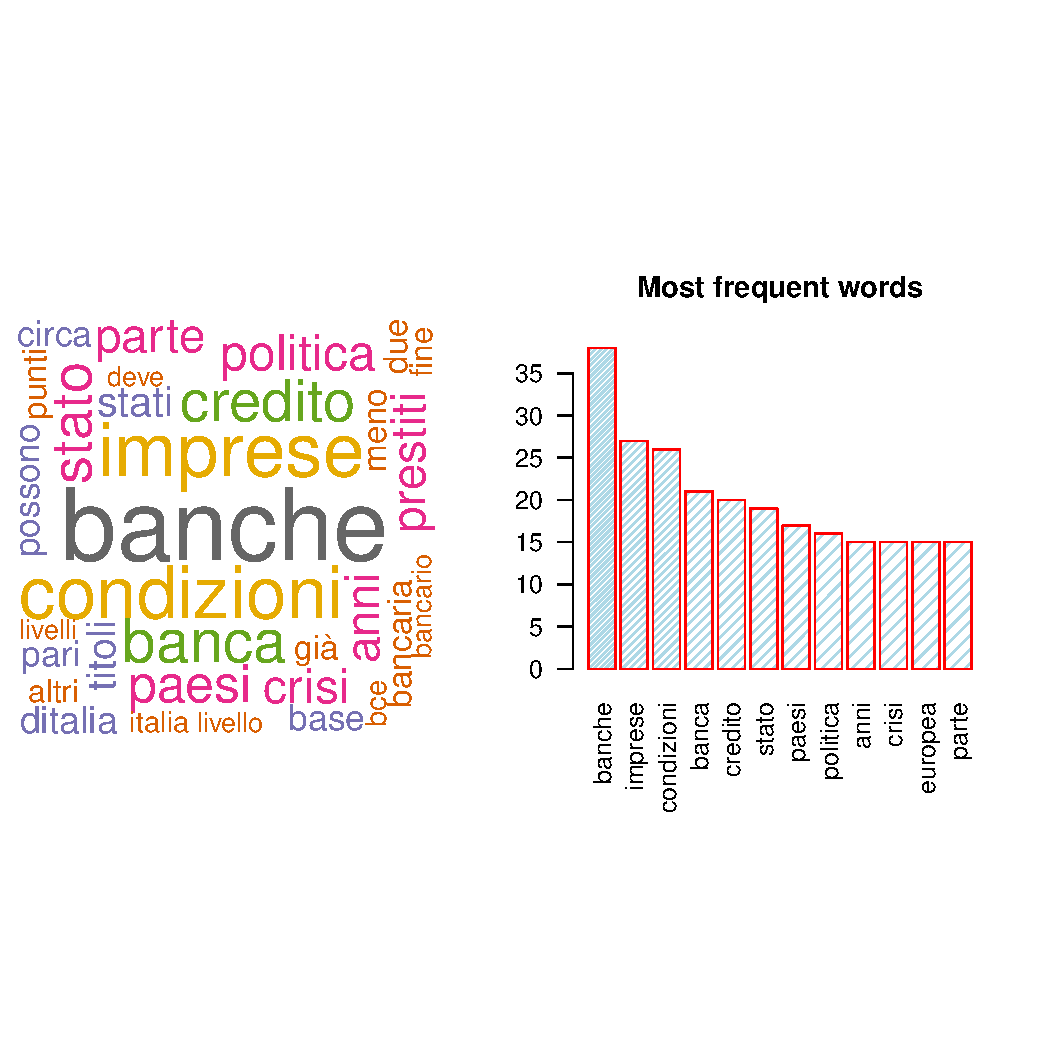
\includegraphics[scale=0.5 , width=13.5cm,height=11.1cm]{WordCloud_nostem2004.pdf}
\vspace{-5\baselineskip} 
\caption{Wordcloud for the "Considerazioni  Finali 2005"  (without stemming)} 
\label{fig:wordcloud05s}
\end{subfigure}\\

\begin{subfigure}{.8\linewidth}
\centering
\includegraphics[scale=0.5 , width=13.5cm,height=11.1cm]{WordCloud_stem2004.pdf}
\vspace{-5\baselineskip} 
\caption{Wordcloud for the "Considerazioni  Finali 2005"  (with stemming)} 
\label{fig:wordcloud05n}
\end{subfigure}
\caption{ }
\label{fig:test32}
\addtocounter{figure}{1}
\end{figure}

\begin{figure}[!htp]
\ContinuedFloat
\begin{subfigure}{.8\linewidth}
\centering
\includegraphics[scale=0.5 , width=13.5cm,height=11.1cm]{WordCloud_nostem2009.pdf}
\vspace{-5\baselineskip} 
\caption{Wordcloud for the "Considerazioni  Finali 2010"  (without stemming)} 
\label{fig:wordcloud10s}

\end{subfigure}\\

\begin{subfigure}{.8\linewidth}
\centering
\includegraphics[scale=0.5 , width=13.5cm,height=11.1cm]{WordCloud_stem2009.pdf}
\vspace{-5\baselineskip} 
\caption{Wordcloud for the "Considerazioni  Finali 2010"  (with stemming)} 
\label{fig:wordcloud10n}
\end{subfigure}
\caption{}
\label{fig:test2}
\addtocounter{figure}{1}
\end{figure}



\begin{figure}[!htp]
\ContinuedFloat
\begin{subfigure}{.8\linewidth}
\centering
%\subfloat[a]{\includegraphics[scale=2.5 , width=13.5cm,height=13cm]{WordCloud_nostem2014.pdf}} \\
\includegraphics[scale=0.8 , width=13.5cm,height=11.1cm]{WordCloud_nostem2014.pdf}
\vspace{-5\baselineskip} 
\caption{Wordcloud for the "Considerazioni  Finali 2015"  (without stemming)} 
\label{fig:wordcloud15s}
\end{subfigure}\\[2ex]

\begin{subfigure}{.8\linewidth}
%\ContinuedFloat
\centering
%\subfloat{\includegraphics[scale=2.5 , width=13.5cm,height=13cm]{WordCloud_stem2014.pdf}}
\includegraphics[scale=0.5 , width=13.5cm,height=11.1cm]{WordCloud_stem2014.pdf}
\vspace{-5\baselineskip} 
\caption{Wordcloud for the "Considerazioni  Finali 2015"  (with stemming)} 
\label{fig:wordcloud15n}
\end{subfigure}
\caption{}
\label{fig:test1}
\addtocounter{figure}{1}
\end{figure}




As examples, the  pictures  \ref{fig:test32}, \ref{fig:test2}  and \ref{fig:test1} show the more relevant
themes considered in the {\it Governor's Concluding Remarks} for the years 2005, 2010 and 2015. For each year,
we show a couple of figures which allow to compare the effect of the stemming on the actual word frequency distribution.  The process of stemming allows to extract the root of the words. The ensuing wordcloud
 provides a more accurate picture of the relative frequency of the word stems. 
From these set of figures we can see how the focus of the words has shifted from the Banks in 2005 to the firms and the State 
in 2010 to arrive, in 2015, to financial system, crises and banks.
Although they don't provide a metric space for numerical comparisons, from a qualitative standpoint reading and interpretation 
of  word-clouds is much faster with respect to the histograms.
 The word-cloud employs the 
technique of tagging for classifying the importance of words. The social media have already extensively used 
the tagging technique as a massively distributed and participative method of expressing emotions and classifying information. 
Here we will
restrict ourselves considering the tagging as a means of classifying the relative importance of words.


\section{An empirical application with a Bank of Italy corpus}
\label{sec:Empirical_application} 
In order check the actual behavior of the available text mining procedures we have taken into account a 
corpus composed of documents relevant for central banking issues. In order to allow comparisons we have chosen
a set of publicly  available  documents. With this goal in mind we have taken the stream of the issues from 1996 to 2015 
of the Bank of Italy {\it Governor's Concluding Remarks} \footnote {In Italian the document is titled: 
{\it Le considerazioni finali}.}. The {\it Concluding Remarks} is a synthesis of the key developments of the economic picture for Italy, the euro 
area and the rest of the world for the previous year and the first quarter of the current year. 
This is a corpus of about $181000$ words and $1.2 MB$ in size. Though of very limited size, this corpus is very helpful in 
 checking and evaluating the analytical tools available in the \proglang{R} package. 
In particular this empirical section has a twofold purpose: 
\begin{itemize}
\item to present the result of some analyses carried out on corpus of documents 
relevant for a Central Bank;
\item to show the suitability of the analytical instruments available on the statistical package \proglang{R};  
\end{itemize}

A very relevant consideration to take into account here is the language of the corpus. As a matter of fact many
computational tools are already quite developed for the English, German and Chinese languages
 while they are still at a rather primitive level for the Italian.\par  
Our approach is somewhat similar to \citet{Moniz2014} who chose to analyze the interest rate minutes 
of the Bank of England in order to design an analytical engine that is able to evaluate and predict the impact of
central bank communication on formation of investors' interest rate expectations. On the other hand,
here we just consider  the linguistic features and the polarity of the sentiment expressed in the texts. \par

%Any kind of text mining and sentiment analysis activities can be broken down as shown in ~\ref{tm_scheme1}

The first analysis consider the word frequency distributions of the documents contained in our corpus.
The following picture shows the frequency distribution of the ranked word frequency and the Vocabulary size
vs number of terms for the corpus of the Bank of Italy {\it Governor's Concluding Remarks}
\input{Zipf_Heaps.tex}

In the following table we show the results of
a two-sample Kolmogorov-Smirnov test on our corpus: 
\begin{enumerate} [label=\arabic* )] 
\item hypothesis test  that the rank-frequency distribution of the corpus is based on the Zipf's nature:

$D = 0.2922$, $p-value < 2.2 \cdot e^{-16}$  

\item hypothesis test  that the Vocabulary size follows the Heaps' distribution:

$D = 0.2$, $p-value = 1$ 
\end{enumerate}
The  first Kolmogorov-Smirnov test rejects the null hypothesis that the our corpus 
follow the Zipf's distribution.
The second test cannot reject the null hypothesis that the Vocabulary size of our
 corpus adheres to the Heaps' distribution. 
 The rejection of the Zipf's hypothesis might be consequence of the limited number of documents 
taken  into account.  

%\subsection{qualitative analysis on the 
Aside from these statistical analysis we have also employed
the following computational linguistic tools:
\begin{itemize}
\item Sentiment analysis;
\item Readability index;
\item Formality index;
\item Memorability index.
\end{itemize}
The previous tasks have been carried out by taking into account the English version of our the corpus.
All the algorithms for carrying out these analyses  have been taken from the \proglang{R} package \pkg{qdap}.
\subsection{Polarity evaluation}
All the previous  analyses have been carried out by splitting the whole
{\it Concluding Remarks} text on its component statements. \par
The algorithm employed to assign a polarity value for each sentence utilizes the
sentiment dictionary proposed in \citet{Huliu2004}. This algorithm builds a context cluster 
for each one of the polarized word \footnote {As default these words belong to a list of about 
6800 words including mainly nouns, adjectives and adverbs.}. A context cluster is simply a bunch of consecutive 
words around a polarized word \footnote{For the English syntax, a context cluster 
defaults to a sequence of 4 words before and two words after the polarized word.}. 
In a context cluster the words  are tagged as neutral $(x_i^0)$, negator $(x_i^N)$,
amplifier $(x_i^a)$, or de-amplifier $(x_i^d)$. 
Neutral words only affect the word count $(n)$. These tagged words 
can act as valence shifters increasing or decreasing the effect of the polarized word. 

% Each polarized word can be given a weight  $w$ based on the weights from the polarity.frame
%argument and then further weighted by the number and position of the valence shifters directly
%surrounding the positive or negative word. The researcher may provide a weight $c$ to be utilized
%with amplifiers/de-amplifiers (default is .8; deamplifier weight is constrained to a  lower bound equal to $ -1$).
In order to get a polarity measure for a given sentence, finally 
the polarity for each context cluster $(x_i^T)$ is achieved by summing  the value of polarized
words and normalizing this sum by the square root of the word count.
\begin{equation}
\delta_i = \frac{x_i^T}{\sqrt{n}}
\end{equation}
where: \\
\begin{equation}
x_i^T = \sum (1+c\cdot (x_i^A-x_i^D))\cdot w \cdot(-1)^{\sum x_i^N}
\end{equation}

$c$ is a weight employed for smoothing the effects of amplifiers or de-amplifiers words, this user-defined 
value defaults to $0.8$, $w=\pm 1$ is the sign of the polarized word.

\begin{equation*}
x_i^A = \sum \left ( w_{neg}\cdot x_i^a \right)
\end{equation*}
\begin{equation*}
x_i^D = \max \left(x_i^{D^\prime}, -1\right)
\end{equation*}

\begin{equation*}
x_i^{D^\prime} = \sum  (-1) \cdot \left( w_{neg}\cdot x_i^a + x_i^d \right)
\end{equation*}
 
and finally 

\begin{equation*}
w_{neg} = \left( \sum x_i^N \right) \mod 2
\end{equation*}
 
This amounts to say  that the polarity for a given context cluster is computed by the algebraic sum of 
amplifiers and de-amplifiers suitably considering the number of negator elements.
 

There exist two main approaches to the problem of extracting sentiment automatically.\par
The first one is a lexicon-based approach which involves calculating orientation for a document from
the semantic orientation of words or phrases in the document (see \citet{Turney2002}). The 
second one is a text
classification approach involves building classifiers from labeled instances of texts or
sentences (\citet{PLeeShiv2002} ), essentially a supervised classification
task. The latter approach could also be described as a statistical or machine-learning
approach. In this empirical application, we have followed the first method in which we employ dictionaries of words annotated
with the word�s semantic orientation, or polarity.

In our empirical application we have evaluated the evolution of the polarity over the flow of the 
{\it Concluding Remarks} of the last twenty years. As example, in the picture \ref{tm_Polarity} we show the polarity
 of  eight of the past issues of the {\it Concluding Remarks}:
\input{Polarity_8pic.tex}
the whole set of eight pictures show a substantial prevalence for a neutrality with a small optimism towards the end of the speech for 
some years.
\subsection{Readability assessment}
Readability assessment provides a measure of the effort required to a reader to understand a text.
Most of the classical readability metrics are linear model of few superficial features of words and sentences.
In our empirical application we have chosen to employ the default function available in the \pkg{qdap} R package for computing 
the automated readability index $ARI$ (\citet{Senter67}). It produces an approximate 
representation of the US grade level needed to comprehend the text.

The formula for calculating the automated readability index $(ARI)$ is given in equation \ref{ARI_equ}:
\begin{equation}
ARI = 4.71 \cdot \left( \frac{N_{char}}{N_{words}}\right) + .5\cdot\left( \frac{N_{words}}{N_{sentences}} \right) - 21.43
\label{ARI_equ}
\end{equation}
where: $N_{char}$ is the total number of characters  in the text,\par \hskip 2em $N_{words}$ is the total number of words and \par
\hskip 2em $N_{sentences}$ is the total number of sentences in the text. \par This index tends to reward the employment of 
short words and short sentences.
ARI is a simple empirical derivation for the English language which provides a useful comparison tool over time and
among different documents belonging to the same class.
In the  picture \ref{tm_Readability} we show the readability evolution   for eight of the past 
issues of the {\it Concluding Remarks},

\input{Readability_8pic.tex}
Values of the ARI index  in the range $12-15$ are usually classified as readable for people with a College degree.

\subsection{Formality assessment}
Another relevant feature allowing to numerically gauge the degree of the context-dependence of a document is the formality of a 
document. There are some different definitions of the for the formality. Here we have chosen the
 the definition suggested in \citet{Helig2002} where the Formality score is calculated according the equation: 
\begin{equation}
F = 50\cdot(\frac {n_f - n_c}{N} + 1 )
\end{equation}

where: $f=\left\{ {nouns, adjective, preposition, article}\right\} $ \hskip  2em  $n_f = \left\vert{f}\right\vert$,\par
 \hskip 3em    $ c=\left\{ {pronoun, adverb, verb, interjection}\right\} $ \hskip 2em $n_c = \left\vert{c}\right\vert$  \par
 \hskip 3em    $ N= \sum (f + c + conjunctions)$

This Formality score gets higher when statements make more use of nouns and adjectives rather than 
pronouns and adverbs.
In the  picture ~\ref{tm_Formality} we show the formality evolution for eight of the past 
issues of the {\it Concluding Remarks},

\input{Formality_8pic.tex}

Reference values for the Formality measure taken from \citet{Helig2002} indicates values of 70 as
highly formal. The last issues of the {\it Concluding Remarks} feature a 
systematically higher values for the Formality index which is in the range $\left[70 \div 75\right]$. This result
confirms our intuition of highly formal documents leaving few room to individual interpretation. 

 
\subsection{Scraping Google search hits}

Because of its aggregation of millions of searches, Google search data features a great potential in tracking 
and forecasting massive social phenomena.  
Google search results can be employed as a useful indicator of public opinion. For example,
 \citet{David2014}, a fellow analyst at Google 
has used search data to research several topics, such as quantifying the effect of racism on the 2008 presidential election. The 
finding was that Obama did worse in states with higher racist query volume.
An arbitrary, though comparable way to measure the interest gained by the issuance of the {\it Concluding Remarks}
 has been devised. The measure is based on the computation of the Google Hits  for each one of the sentences contained 
in the considered document.
The memorability of eight of the past issues of the {\it Concluding Remarks} is shown in the figure \ref{tm_Memorability}:

\input{Memorab_8pic.tex}

Memorability is expressed as natural logarithms. Values in the range $12-13$ mean that each sentence has a {\it Google-like} popularity of
\begin{equation} 
e^{12} \le Google_{popularity} \le e^{13} \quad \to \quad  162000 \le Google_{popularity} \le 443000
\end{equation}
Timing considerations are quite relevant for these results. Here we have tallied these {\it google hits} for statements 
the are partially repeated and span a very wide time interval. To provide an approximate form of a yardstick,
we have applied the same measurement to the following two analogous documents:
\begin{enumerate} [label=\arabic* )]
\item The Federal Reserve Board {\it Semiannual Monetary Policy Report to the Congress} held on July 15, 2015;
\item The European Central Bank {\it Account of the monetary policy meeting of the Governing Council of the E.C.B.} held on
October 22, 2015; \footnote{These documents can be found respectively at 
http://www.federalreserve.gov/newsevents/testimony/yellen20150715a.htm 
and https://www.ecb.europa.eu/press/accounts/2015/html/mg151119.en.html}
\end{enumerate}
The figure \ref{Google_Memorability} provides a quick description of the analysis on these documents. 
\input{Memorab_compar_2pic.tex} 
Even if the behavior of the two curves is quite different and the {\it Google} measured 
popularity seems higher for the Federal Reserve Board testimony, the shown numbers go from 10 to 13 and therefore are very close 
to those achieved by the considered {\it Concluding Remarks}. 
These results should be used to further dig up specialized press releases in order to evaluate some form of impact of the 
news on other financial agents.

 
\section{Concluding Remarks}
\label{sec:Conclusion} 

In this paper we have presented the main computational linguistic methodologies for mining 
the relevant information from a corpus of documents and evaluating some  summary statistics. 
These methodologies employ a tool-set taken from the information retrieval technology.\par
We have shown that these technologies can be quite helpful in quickly analyzing
huge amount of documents and automatically extracting  sentiment or opinion orientation and
gauging polarity of these sentiments.   
By taking advantage of some packages available on the 
CRAN\footnote{Comprehensive R Archive Network, https://cran-r-project.org}} repository,  we have written some \proglang{R} procedures  implementing different algorithms for text mining and sentiment
analysis. These \proglang{R} procedures have been applied for the analysis of an 
homogenous corpus of  documents based of the Bank of Italy {\it Governor's concluding Remarks} 
of the last 20 years.\par  The main conclusions are:
\begin{enumerate}  [label=\arabic* )]
\item the consideration of the last 20 editions of the {\it Concluding remarks} has shown us that these
documents tend to stay pretty much neutral over all the extension of the speech. 
The results of these analyses allow to trace back the sentiment shift over time in relation to the 
different short term economic conditions.\par
\item The $ARI$ readability index shows a readability in the range $12-15$ which approximately implies a college degree.\par 
\item The examined corpus of documents, as it could be expected, has shown a quite high average level of the Formality score.
\item The English versions of the {\it Concluding Remarks} have shown a number of hits in the
the range $10^5$. This measure is comparable with that achieved with similar reports from 
the ECB and the FRB.
\end{enumerate}
The present strand of research looks quite promising especially for the possibility to quickly
provide institutional answers more closely connected to the social emotions and preferences of the different economic agents.


%% references can alternatively be entered by hand
%\nocite{ref_HeMa}
\bibliographystyle{chicago}
\bibliography{user2015bib}
%\subsubsection*{References}

%\begin{hangparas}{.25in}{1}
%AuthorA (2007). Title of a web resource, \url{http://url/of/resource/}.


\end{document}
